\documentclass[conference]{IEEEtran}
\IEEEoverridecommandlockouts

\usepackage{cite}
\usepackage{tabularx}
\usepackage{booktabs}
\usepackage{amsmath,amssymb,amsfonts}
\usepackage{algorithmic}
\usepackage{graphicx}
\usepackage{textcomp}
\usepackage{xcolor}


\def\BibTeX{{\rm B\kern-.05em{\sc i\kern-.025em b}\kern-.08em
    T\kern-.1667em\lower.7ex\hbox{E}\kern-.125emX}}

\begin{document}

\title{Detección y Clasificación Explicable de Manchas Solares Mediante Aprendizaje Profundo y XAI}


\author{
    \IEEEauthorblockN{Ignacio Martínez Hernández}
    \IEEEauthorblockA{\textit{Doctorado Sistemas en Ingeniería},
        \textit{Universidad de Talca},
        Talca, Chile,
        imartinez17@alumnos.utalca.cl}
}

\maketitle


\begin{IEEEkeywords}
    Visión computacional, Explicabilidad (XAI), Manchas solares, Aprendizaje profundo, Clasificación McIntosh.
\end{IEEEkeywords}



\section*{Contexto}
Las manchas solares son regiones oscuras y temporales en la superficie del Sol, caracterizadas por una temperatura más baja que sus alrededores. Son causadas por la actividad magnética del Sol, donde fuertes campos magnéticos inhiben el flujo de calor desde el interior solar. El estudio de las manchas solares es crucial para comprender el ciclo solar y su impacto en el clima espacial y las comunicaciones terrestres.

\section*{Planteamiento del Problema}

%Actualmente, la detección y clasificación de manchas solares depende de expertos humanos. Este proceso es lento, subjetivo y difícil de escalar. Además, existe poca explicabilidad en los sistemas automáticos existentes, lo que dificulta su adopción en astronomía profesional.
La detección y clasificación de manchas solares, realizada tradicionalmente por expertos humanos, es un proceso inherentemente lento, susceptible a la subjetividad y difícil de escalar ante el creciente volumen de datos astronómicos. Para abordar estas limitaciones, se han desarrollado sistemas automáticos, a menudo basados en aprendizaje profundo. Sin embargo, una barrera significativa para la adopción generalizada de estos sistemas en la astronomía profesional es su limitada explicabilidad; es decir, estos algoritmos no suelen ofrecer una justificación clara de por qué llegan a una determinada conclusión (por qué una región es identificada como mancha solar o por qué una mancha se clasifica de cierta manera según McIntosh).
La explicabilidad (XAI, por sus siglas en inglés, Explainable Artificial Intelligence) se refiere a la capacidad de un sistema de inteligencia artificial para proporcionar una comprensión clara y comprensible de sus decisiones o predicciones. En el contexto de la detección y clasificación de manchas solares, la XAI es crucial. Permite a los astrónomos y físicos solares no solo confiar en las predicciones de los modelos, sino también entender los factores determinantes detrás de ellas. Esto es vital para validar los resultados del modelo contra el conocimiento físico existente, descubrir nuevos patrones o correlaciones que el modelo podría haber aprendido de los datos, y facilitar la integración de estas herramientas en la investigación científica y operativa, donde la transparencia y la interpretabilidad son fundamentales. La carencia de esta transparencia en muchos sistemas automáticos actuales dificulta su plena aceptación y aprovechamiento por la comunidad científica.

\section*{Propuesta de Solución}

Un sistema que combina:
\begin{enumerate}
    \item \textbf{Detección con YOLO}: Localización de regiones de interés (ROIs) que contienen manchas solares.
    \item \textbf{Clasificación con ResNet}: Categorización precisa de las manchas detectadas según el esquema de clases McIntosh.
    \item \textbf{Explicabilidad con LLM}: Generación de reportes detallados que explican las decisiones de clasificación (por qué una mancha solar recibe una determinada clase McIntosh), vinculando las características identificadas por el modelo.
\end{enumerate}


\section*{Metodología}

\subsection*{Adquisición de Datos}
\begin{itemize}
    \item Fuente primaria: Imágenes de satélites solares (Solar Dynamics Observatory, SDO)
    \item Etiquetado: Realizado por expertos y/o validado contra catálogos existentes (NOAA, Debrecen Photoheliographic Data), o dataset utilizado en algún articulo de referencia con otras técnicas de detección y clasificación.
\end{itemize}


\subsection*{Preprocesamiento}
Se realizará una investigación de las técnicas de preprocesamiento empleadas en los métodos actuales y el estado del arte para la detección y clasificación de manchas solares. El objetivo es identificar y aplicar aquellas transformaciones que demuestren ser beneficiosas para el rendimiento de los modelos, evitando pasos innecesarios o potencialmente contraproducentes. Entre las técnicas a considerar, se evaluará la pertinencia de:
\begin{itemize}
    \item Normalización de contraste y brillo para estandarizar las condiciones de las imágenes.
    \item Técnicas de aumento de datos (rotaciones, escalado, variaciones de brillo/contraste), si se determina que son necesarias para mejorar la generalización del modelo, especialmente en casos de conjuntos de datos limitados o desbalanceados.
    \item Extracción y preparación de Regiones de Interés (ROIs) a partir de las detecciones iniciales para optimizar la entrada a la fase de clasificación.
\end{itemize}
La selección final de las técnicas de preprocesamiento se basará en la evidencia de su efectividad en contextos similares y su impacto positivo en las métricas de evaluación.

\subsection*{Modelado}
\begin{itemize}
    \item \textbf{Fase 1 (Detección)}:
          \begin{itemize}
              \item Arquitectura YOLO con fine-tuning para dominio solar.
              \item Salida: Coordenadas (bounding boxes) de las regiones candidatas a contener manchas solares.
          \end{itemize}
    \item \textbf{Fase 2 (Clasificación)}:
          \begin{itemize}
              \item ResNet para categorización McIntosh.
              \item Entrada: ROIs recortadas y preprocesadas obtenidas de la fase de detección.
          \end{itemize}
    \item \textbf{Fase 3 (Explicabilidad)}:
          \begin{itemize}
              \item Modelo de Lenguaje Grande (LLM) (un modelo de la familia GPT o similar) que recibirá como entrada:
                    \begin{itemize}
                        \item La imagen de la Región de Interés (ROI) de la mancha solar clasificada.
                        \item La predicción de la clase McIntosh asignada por el modelo ResNet.
                        \item Mapas de activación de clase (Grad-CAM) que visualizan las regiones de la imagen más relevantes para la decisión del modelo de clasificación.
                        \item Valores de importancia de características (SHAP) que indican la contribución de diferentes aspectos de la imagen a la predicción.
                    \end{itemize}
              \item Salida: Un reporte textual generado por el LLM que explique, de manera interpretable, por qué la mancha solar fue asignada a una determinada clase McIntosh, basándose en la evidencia visual y las salidas de las técnicas XAI.
          \end{itemize}
\end{itemize}

\subsection*{Explicabilidad}
La explicabilidad se generará combinando técnicas de XAI visual, como Grad-CAM, y de atribución de características, como SHAP, para identificar las regiones y aspectos de la imagen más relevantes para la clasificación McIntosh realizada por el modelo ResNet. Estas salidas, junto con la imagen de la mancha solar y su clasificación predicha, alimentarán un Modelo de Lenguaje Grande (LLM). El LLM producirá un reporte textual que articule, de forma interpretable, por qué se asignó una clase específica. Este reporte facilitará la validación física por parte de expertos, permitiéndoles evaluar la coherencia del razonamiento del modelo con el conocimiento solar existente y fomentando la confianza en el sistema.


\subsection*{Validación}
\begin{itemize}
    \item Métricas cuantitativas: mAP (detección), precisión/recall (clasificación)
    \item Evaluación cualitativa: Encuestas a expertos sobre utilidad de explicaciones
    \item Comparación con líneas base tradicionales
\end{itemize}


\begin{figure}[ht]
    \centering
    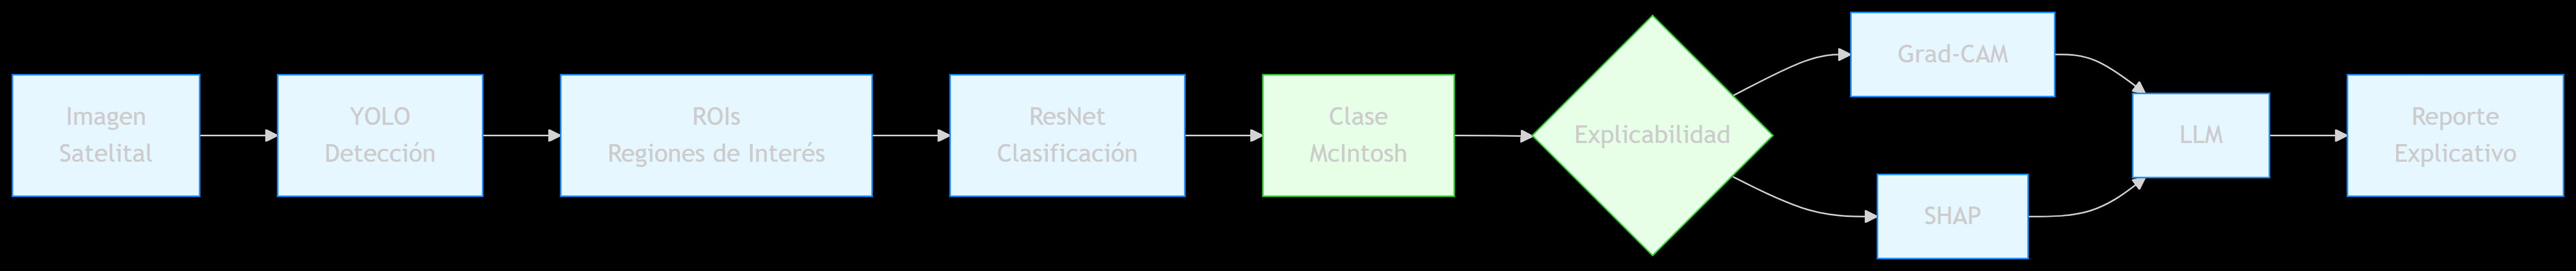
\includegraphics[width=0.48\textwidth]{diagrama_metodologia-2.png}
    \caption{Diagrama de la metodología propuesta para la detección, clasificación y explicabilidad de manchas solares.}
    \label{fig:metodologia}
\end{figure}

\section*{Resultados Esperados}
\begin{enumerate}
    \item Pipeline funcional que integre detección-clasificación-explicabilidad
    \item Métricas competitivas con estado del arte en ambos módulos de visión
    \item Explicaciones coherentes con conocimiento físico establecido
\end{enumerate}


\section*{Impacto}

Si bien existen algoritmos y modelos de inteligencia artificial capaces de detectar y clasificar manchas solares, una limitación común es la falta de transparencia en sus procesos de toma de decisiones. El principal impacto de este trabajo radica en la integración de un componente de Inteligencia Artificial Explicable (XAI) diseñado para generar justificaciones interpretables de las clasificaciones.
El sistema propuesto no solo identificará y clasificará las manchas solares según el esquema McIntosh, sino que, a través de un LLM, buscará explicar por qué una mancha solar recibe una clasificación específica.

\section*{Conclusión}
Este trabajo propone un enfoque integrado para el análisis automatizado de manchas solares, priorizando la transparencia interpretativa mediante XAI. La arquitectura modular permite mejoras iterativas en cada componente. Futuras líneas explorarán el uso de datos multiespectrales y adaptación a sistemas de alerta temprana.

\end{document}